\documentclass[a4paper]{article}
\usepackage{geometry}
\usepackage{graphicx}
\usepackage{caption}
\usepackage{booktabs}
\usepackage{fancyhdr}
\usepackage{url} % Adicionado para suportar \url

\geometry{margin=1in}

\pagestyle{fancy}
\fancyhf{}
\fancyhead[C]{Análise Instagram - 7 de Outubro 2018}
\fancyfoot[C]{\thepage}

\begin{document}

\begin{titlepage}
    \centering
    \vspace*{2cm}
    {\Huge\bfseries Análise Instagram\\7 de Outubro 2018\par}
    \vspace{1cm}
    {\Large Israel - DoE Atividade 1\par}
    \vspace{2cm}
    {\large \today\par}
\end{titlepage}

\section{Pré-processamento dos Dados}
Esta análise foca em um subconjunto dos dados, priorizando o dia 7 de outubro de 2018, primeiro turno das eleições, para reduzir a carga de memória. Os dados foram processados com Pandas, totalizando 529.218 linhas e 15 colunas. Foram identificados valores nulos em \texttt{comment\_tag} (1) e \texttt{parent\_comment\_id} (461.023), e todas as datas foram convertidas para o formato \texttt{datetime}. \\ \\

Código completo disponível em \url{https://github.com/imdoamaral/DoE-Atividade-1}.

\newpage

\section{Análise Exploratória}
\subsection{Distribuição de Frequência e Estatísticas Descritivas}
\begin{table}[htbp]
    \centering
    \caption{Estatísticas - Publicações e Comentários por Hora}
    \begin{tabular}{lrr}
        \toprule
        \textbf{Métrica} & \textbf{Publicações} & \textbf{Comentários} \\
        \midrule
        Média & 36,67 & 13.763,46 \\
        Mediana & 25,50 & 13.118,50 \\
        Moda & 3,00 & 1.369,00 \\
        \bottomrule
    \end{tabular}
\end{table}

\textbf{Insight}: A maioria das horas tem poucas publicações (moda 3), mas há picos altos (média 36,67).

\begin{figure}[htbp]
    \centering
    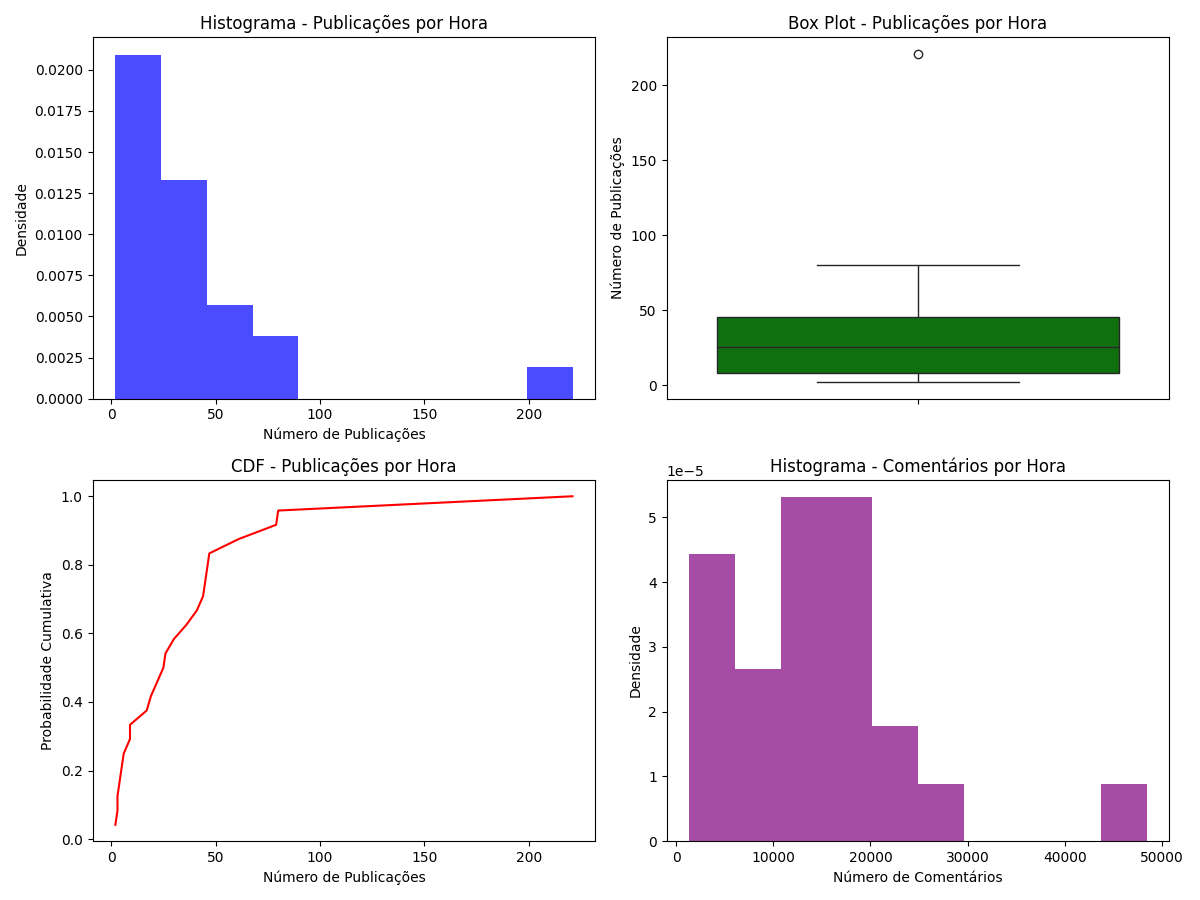
\includegraphics[width=\textwidth]{instagram_exploratory_analysis_subset.png}
    \caption{Histograma de publicações por hora.}
\end{figure}

\textbf{Insights Gráficos}:
\begin{itemize}
    \item \textbf{Histograma - Publicações}: Atividade concentrada em poucas horas.
    \item \textbf{Box Plot - Publicações}: Metade das horas tem até 25 publicações, mas outliers chegam a 219.
    \item \textbf{CDF - Publicações}: Sobe lentamente no começo porque muitas horas tem poucos publicações.
    \item \textbf{Histograma - Comentários}: Picos até 48.415 sugerem grande engajamento em horários específicos, provavelmente ligados a eventos noturnos.
\end{itemize}

\

\subsection{Análise Temporal}
\begin{center}
    \captionof{table}{Picos de Atividade (Top 3)}
    \begin{tabular}{lrr}
        \toprule
        \textbf{Horário} & \textbf{Publicações} & \textbf{Comentários} \\
        \midrule
        00:00 & 240 & 12.258 \\
        15:00 & 88 & 17.841 \\
        23:00 & - & 48.415 \\
        \bottomrule
    \end{tabular}
\end{center}

\textbf{Insight}: Publicações tiveram pico de 240 às 00:00 e 88 às 15:00, com mais atividade no início e meio do dia. Comentários tiveram pico de 48.415 às 23:00, crescendo ao longo do dia com mais engajamento à noite.

\begin{figure}[htbp]
    \centering
    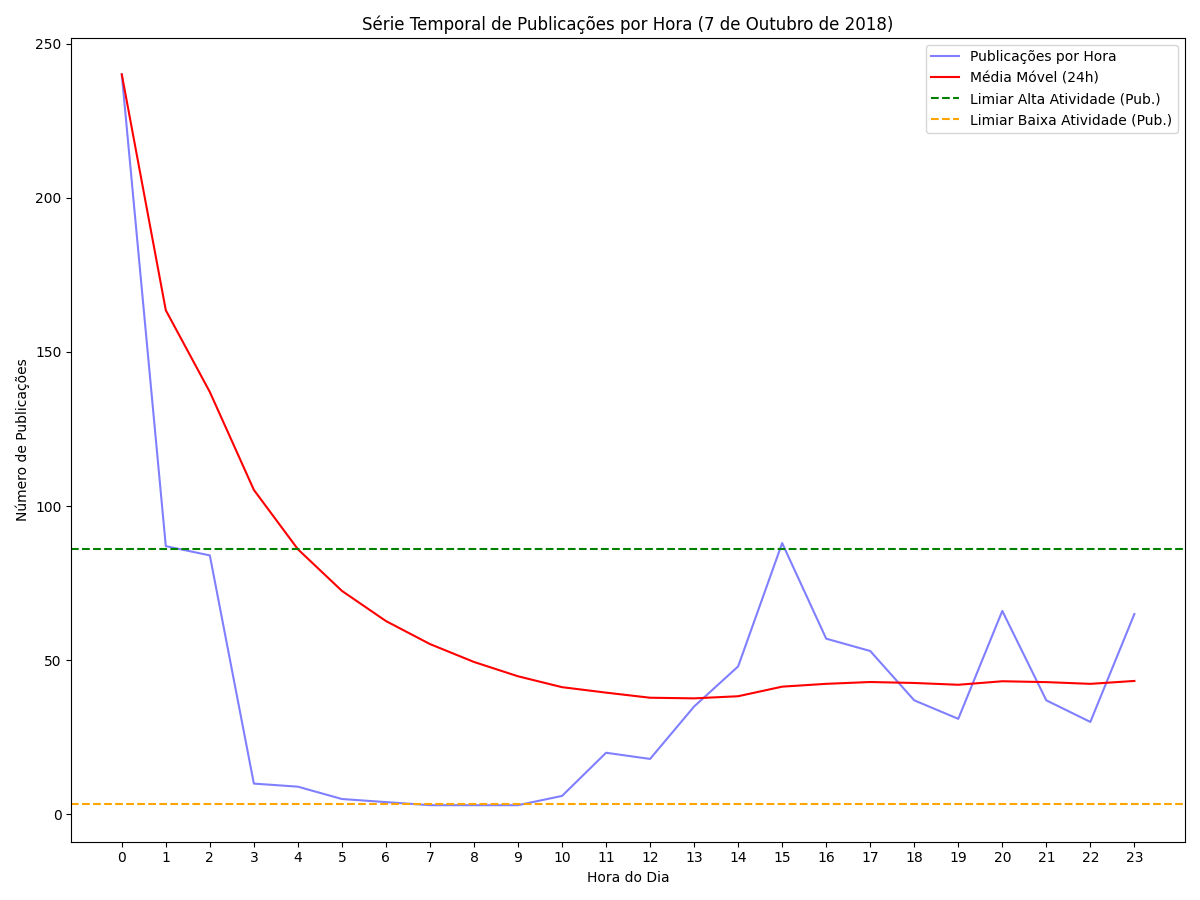
\includegraphics[width=\textwidth]{serie_temporal_publicacoes.png}
    \caption{Série temporal de publicações por hora.}
\end{figure}

\begin{figure}[htbp]
    \centering
    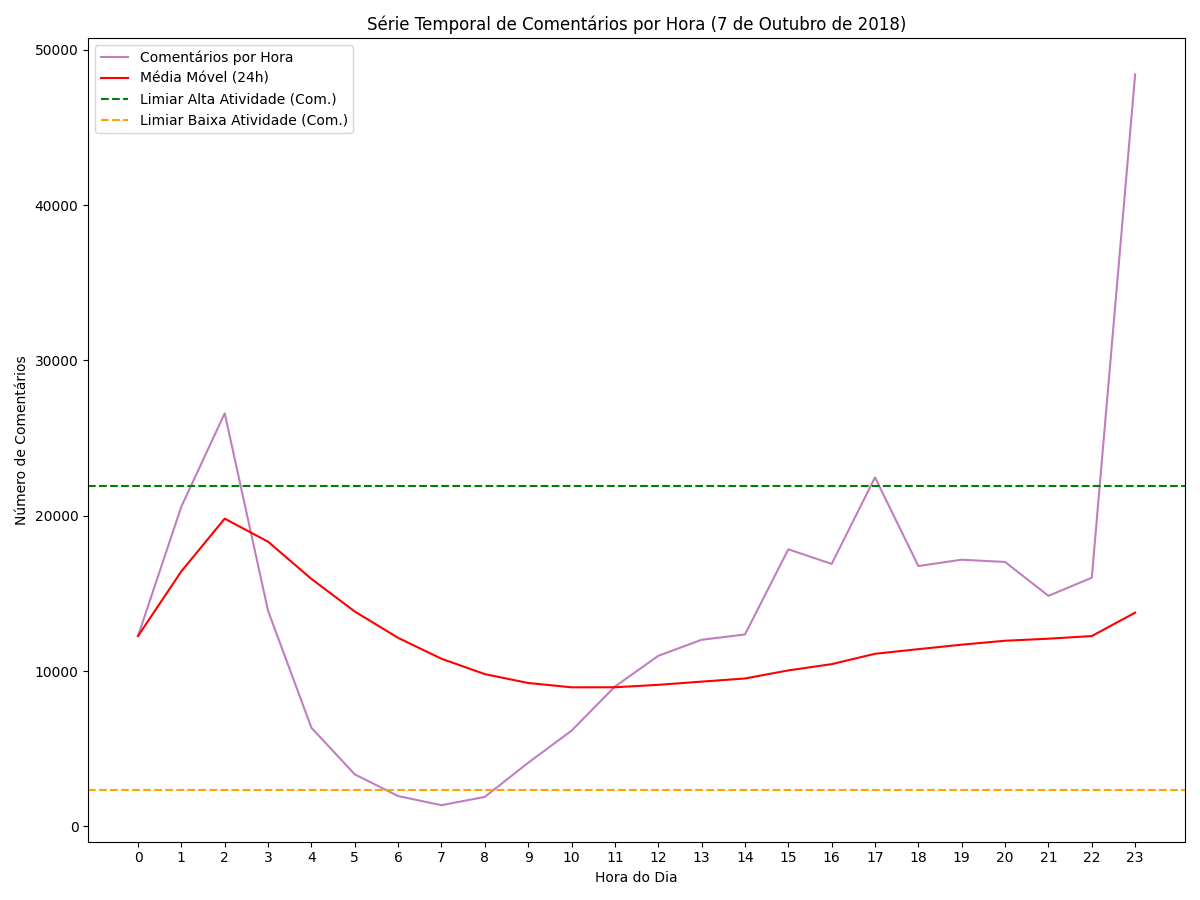
\includegraphics[width=\textwidth]{serie_temporal_comentarios.png}
    \caption{Série temporal de comentários por hora.}
\end{figure}

\subsection{Análise dos Usuários}
\begin{table}[htbp]
    \centering
    \caption{Estatísticas dos Usuários}
    \begin{tabular}{lrr}
        \toprule
        \textbf{Métrica} & \textbf{Publicações} & \textbf{Comentários Recebidos} \\
        \midrule
        Média & 1,93 & 1.359,57 \\
        Mediana & 1,00 & 118,00 \\
        Moda & 1,00 & 4,00 \\
        \bottomrule
    \end{tabular}
\end{table}

\begin{figure}[htbp]
    \centering
    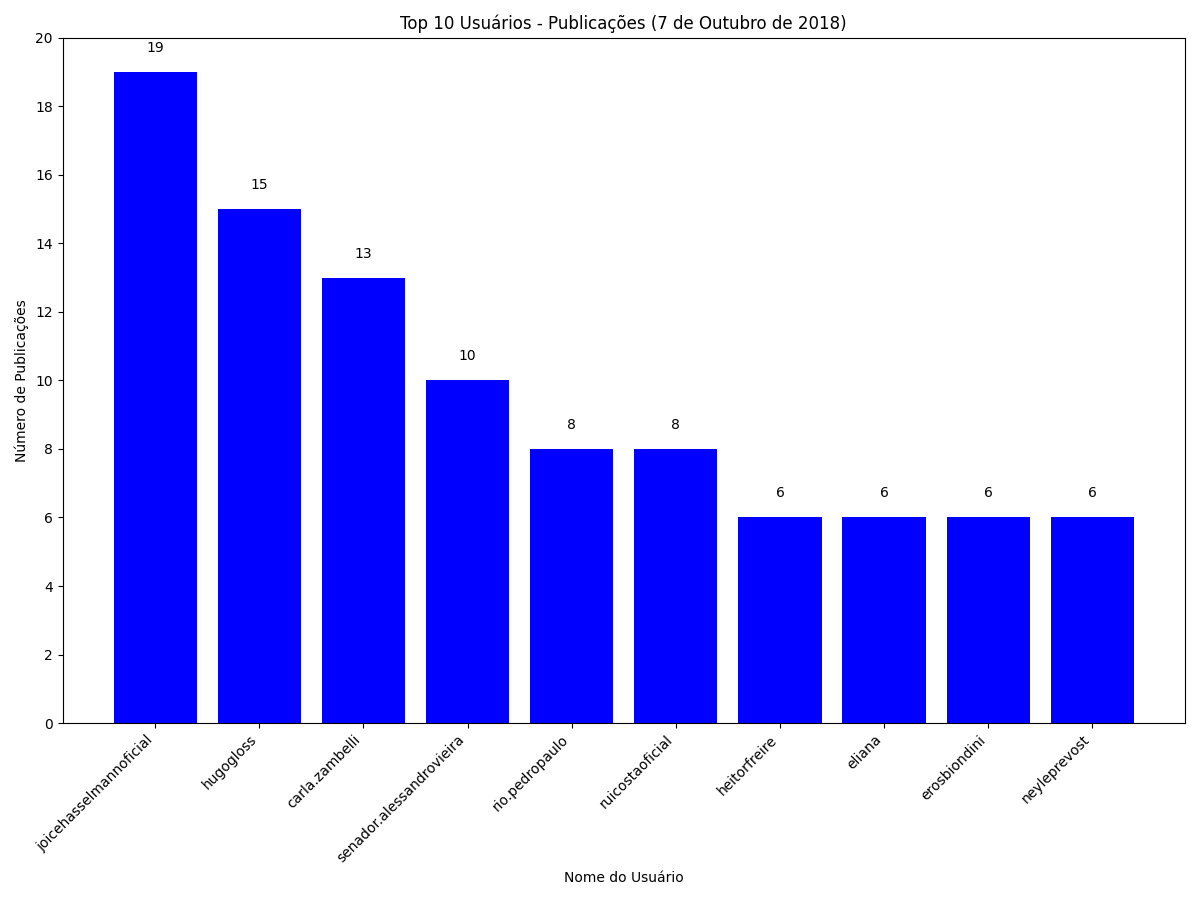
\includegraphics[width=\textwidth]{top_usuarios_publicacoes.png}
    \caption{Usuários mais ativos (publicações).}
\end{figure}

\textbf{Insight (Publicações)}: A maioria fez 1 post (moda 1), alguns até 18.

\begin{figure}[htbp]
    \centering
    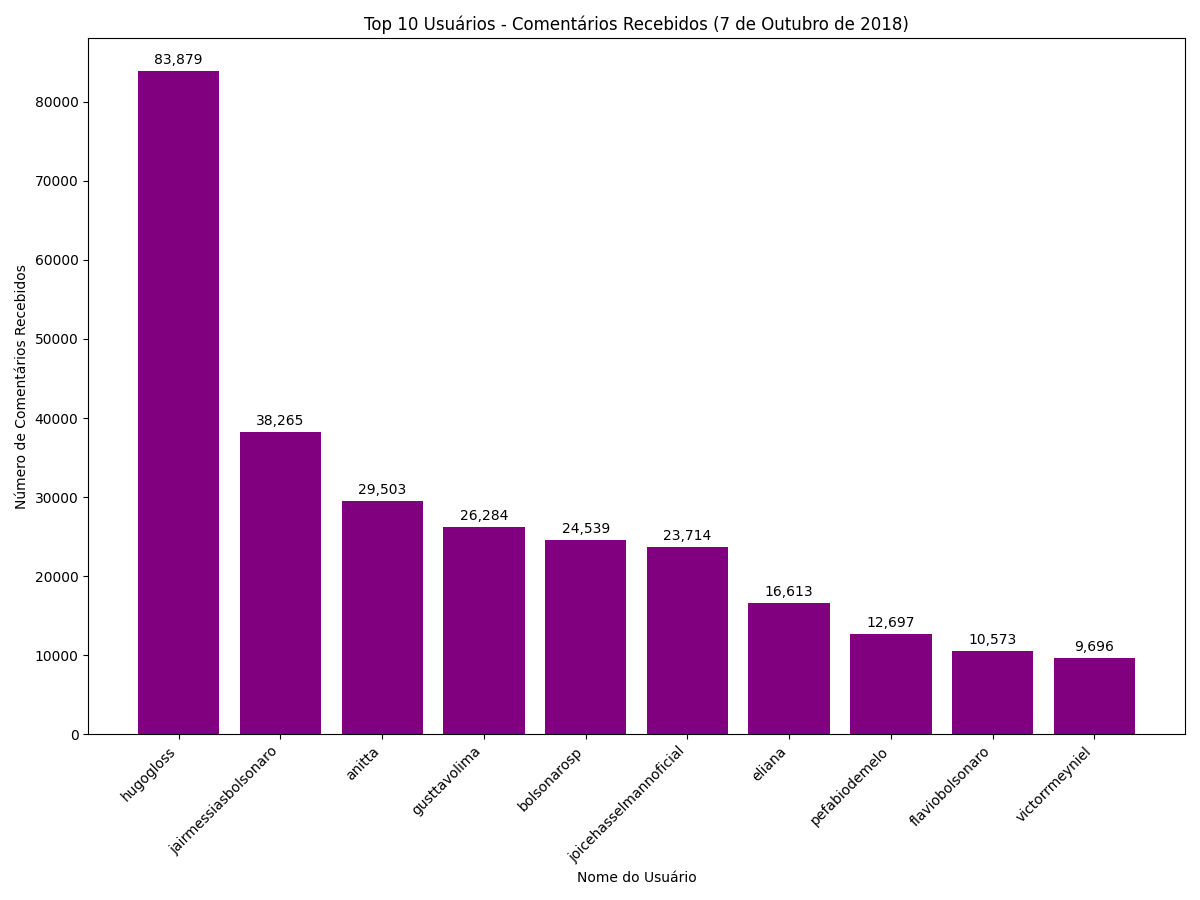
\includegraphics[width=\textwidth]{top_usuarios_comentarios.png}
    \caption{Usuários com mais comentários recebidos.}
\end{figure}

\textbf{Insight (Comentários)}: A maioria recebeu poucos (moda 4), um até 83.878.

\end{document}